\section{Introduction}

Decision Transformers make return a prompt \citep{chen2021decision}. Given a desired return-to-go, a sequence model predicts actions conditioned on the trajectory prefix and the requested future return. This framing is attractive because it turns policy improvement into a simple inference-time interface: request a larger return, sample continuations, and keep a candidate that appears to satisfy the prompt.

That interface also creates a trap. In offline reinforcement learning, the data distribution is part of the problem statement: targets beyond the behavior support are extrapolations, not merely ambitious goals \citep{levine2020offline,fu2021d4rl}. Candidate-count selection amplifies whichever tail the scoring rule prefers. If the selected score is a proxy $\score$ and the deployed objective is real utility $\utility$, increasing the candidate count improves utility only when the high-$\score$ tail is also high-$\utility$. When high target returns move a return-conditioned model outside offline support, the high-score tail can instead contain trajectories whose predicted return is plausible to the model and costly under the real objective.

This paper studies that mechanism in a controlled setting. We deliberately separate the internal/proxy return $\score$ from real utility $\utility$, train a small learned Decision Transformer-style policy on synthetic offline trajectories with limited high-return support, and evaluate top-score selection under in-support, edge-support, and out-of-support return prompts. The goal is not benchmark dominance. The goal is a precise account of when selected return is evidence of utility and when it is a return-conditioning fantasy.

\paragraph{Contributions.}
First, we give a tie-aware finite-pool accounting identity that groups candidates by score level and computes selected real-utility expectation under top-score selection.
Second, we introduce two diagnostics: the Return Fantasy Microscope, which reports prompt-satisfaction, support, and real-utility gaps, and the Tail Phase Diagram, which classifies whether candidate-count pressure helps, saturates, or hurts as $N$ grows.
Third, we provide a learned DT-style synthetic study in which out-of-support target returns create the intended failure: naive top-score selection increases selected proxy return from $9.299$ to $9.468$ while real utility decreases from $7.825$ to $7.381$ between $N=1$ and $N=64$.
Fourth, we evaluate controls and repairs. In-support selection improves real utility; an anti-aligned scorer hurts it; behavior-likelihood and pilot real-utility calibration recover much of the lost utility in the out-of-support condition.
Finally, we include a claim audit that treats the study as a controlled v1: it supports the mechanism claims above and leaves benchmark-scale validation for future work.

\begin{figure}[t]
  \centering
  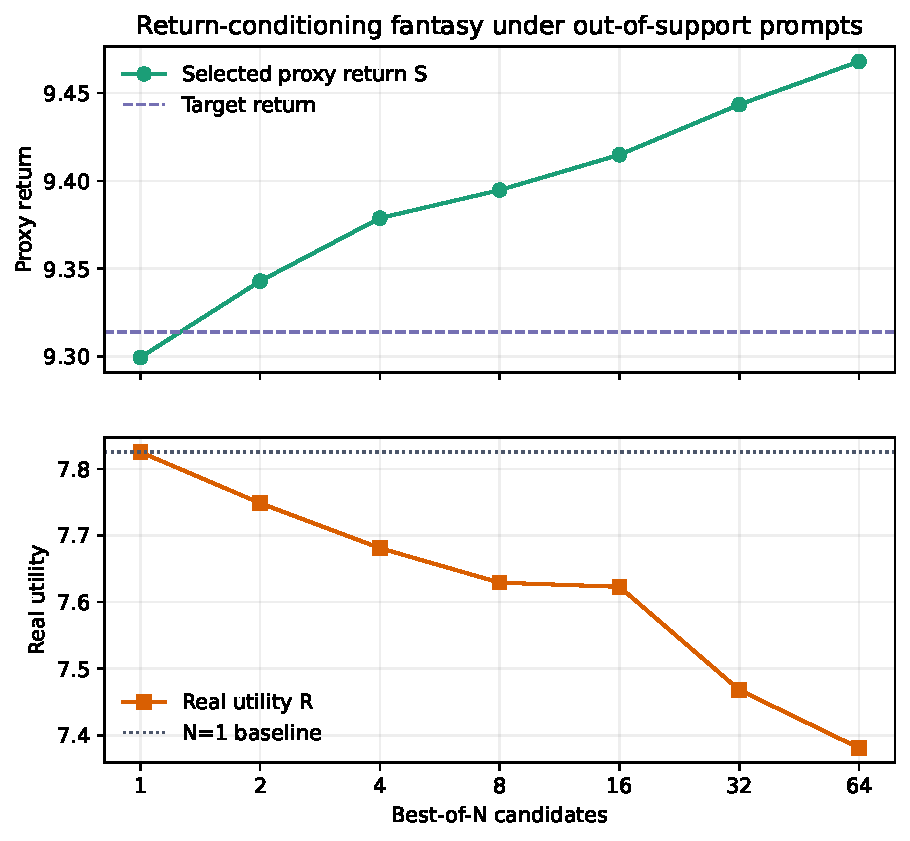
\includegraphics[width=0.94\linewidth]{figures/return_conditioning_fantasy.pdf}
  \caption{\textbf{Return-conditioning fantasy under an out-of-support target.} Naive top-score selection increases selected proxy return $\score$ as candidate count grows, but real utility $\utility$ drops. The offline support boundary is at the empirical $q_{95}=6.314$, while the requested out-of-support return is $9.314$.}
  \label{fig:fantasy}
\end{figure}
